%%%%%%%%%%%%%%%%%%%%%%%%%%%%%%%%%%%%%%%%%
% Medium Length Professional CV
% LaTeX Template
% Version 2.0 (8/5/13)
%
% This template has been downloaded from:
% http://www.LaTeXTemplates.com
%
% Original author:
% Trey Hunner (http://www.treyhunner.com/)
%
% Important note:
% This template requires the resume.cls file to be in the same directory as the
% .tex file. The resume.cls file provides the resume style used for structuring the
% document.
%
%%%%%%%%%%%%%%%%%%%%%%%%%%%%%%%%%%%%%%%%%

%----------------------------------------------------------------------------------------
%	PACKAGES AND OTHER DOCUMENT CONFIGURATIONS
%----------------------------------------------------------------------------------------

\documentclass{resume} % Use the custom resume.cls style

\usepackage[left=0.75in,top=0.6in,right=0.75in,bottom=0.6in]{geometry} % Document margins
\usepackage{hyperref}
\usepackage{array} 
\usepackage{textpos}
\usepackage{graphicx}

\begin{textblock}{7}(0, 0.05)
{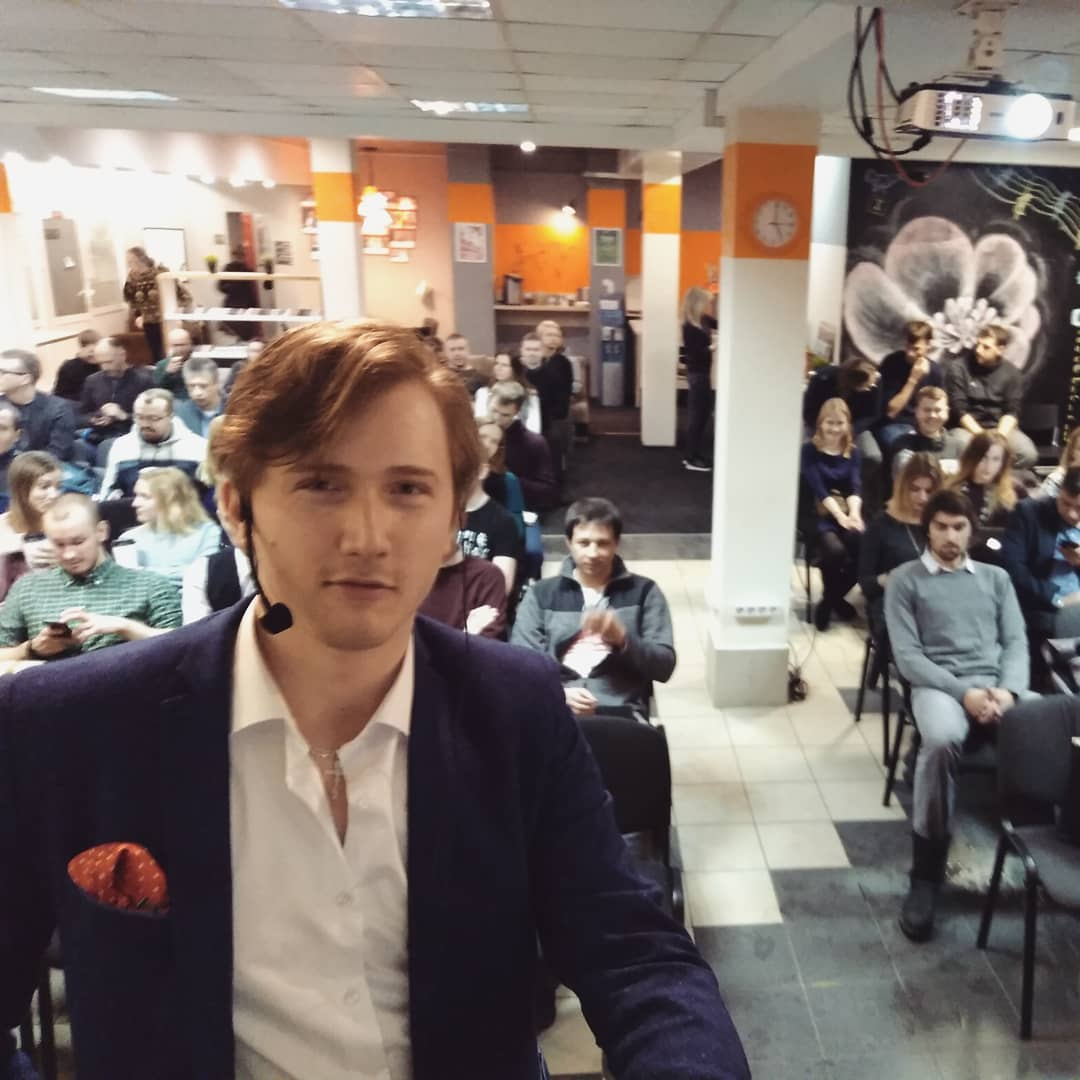
\includegraphics[width=.2\linewidth]{photo.jpg}}
\end{textblock}

\name{Alexander Mikhalchenko} % Your name
\address{Belarus, Minsk 220113} % Your address
\address{+37525$\cdot$951$\cdot$48$\cdot$81 \\ alexander.a.mikhalchenko@gmail.com \\ skype:strrife } % Your phone number and email
\address{https://www.linkedin.com/pub/alexander-mikhalchenko/84/70b/357}

\begin{document}

%----------------------------------------------------------------------------------------
%	SUMMARY SECTION
%----------------------------------------------------------------------------------------

\begin{rSection}{Summary}

I'm skilled fast-learning developer with a strong mathematical background. Over the past years I have worked with a variety of web technologies and I'm experenced in backend (NodeJS, PHP), frontend (Javascript ES5, ES6, Angular, Aurelia, React), databases (MySQL, MongoDB, Redis) and Software architecture. I have good communication skills and ~2 years of working in different teams.

I'm constantly looking for ways to apply and enrich my knowledge. 

Lookig forward to hearing from you!

\end{rSection}


%----------------------------------------------------------------------------------------
%	TECHNICAL STRENGTHS SECTION
%----------------------------------------------------------------------------------------

\begin{rSection}{Technical Strengths}

\begin{tabular}{ @{} >{\bfseries}l @{\hspace{6ex}} l }
JavaScript (3 years) & ES5.1, ES6; Angular, Aurelia, JSPM, Bower, jQuery, React \\
PHP 5.3+ (2 years) & PHP7, Symfony 2, Symfony 1.4, Wordpress, Silex, Composer \\
NodeJS (1 year) & Express, NPM, Grunt, Gulp, Yeoman, Browserify \\
MySQL (2 years) & InnoDB; Raw and with ORMs; Doctrine, PDO \\
NoSQL: MongoDB, Redis (1 year) & ElasticSearch, Mongoose, MapReduce \\
HTML/XML (3 years) & HTML5, DOM, Canvas \\
CSS/SASS/LESS (2 years) & CSS3, Bootstrap, Flat UI \\
Testing & Mocha, Karma, Selenium, PHPUnit, Nightmare.js \\
AWS & EC, S3, SQS  \\
Other Languages & Python (worked with OpenCV), Java, C/C++ \\
VCS & Git, Perforce \\
\end{tabular}

\end{rSection}

%----------------------------------------------------------------------------------------
%	EDUCATION SECTION
%----------------------------------------------------------------------------------------

\begin{rSection}{Education}

{\bf Belarussian State University, Belarus} \hfill {\em 2012 $-$ Present} \\ 
Bachelor Degree in Computer Science \& Mathematics \\
Minor in Intelligent Control Systems \smallskip \\
Courses taken: Algorithms and Data structures, Operating Systems, Calculus, etc. \smallskip \\
Average: 9.47

{\bf Belarussian State University Lyceum, Belarus} \hfill {\em 2010 $-$ 2012} \\ 
Associate degree in Mathematics \\
Average: 9.8

\end{rSection}

%----------------------------------------------------------------------------------------
%	WORK EXPERIENCE SECTION
%----------------------------------------------------------------------------------------

\begin{rSection}{Experience}

\begin{rSubsection}{DualLab}{August 2015 - Present}{Full stack Web Developer}{Minsk, Belarus}
\item Development of the web client and the REST API layer on top of the legacy SOAP API
\item NodeJS + Express used for backend; Angular for frontend
\item Nightmare.js and Mocha for testing
\item Test-driven development
\item Agile Software Development (Scrum)
\item Recommendations from my team leader and colleagues can be found on my \href{https://www.linkedin.com/pub/alexander-mikhalchenko/84/70b/357}{linkedin profile}
\end{rSubsection}

\clearpage


%------------------------------------------------

\begin{rSubsection}{StarOfService}{April 2014 - August 2015}{Full stack Web Developer}{Paris, France}
\item back-end development (PHP, Symfony 1.4)
\item integration with AWS (SQS in perticular)
\item data analysis \& Mixpanel integration
\item the TF-IDF based search engine for the homepage
\item developing from scratch and maintaining the REST API for the iPhone app 
\item backend request moderaton tool
\item front-end development (Angular/jQuery)
\item Agile Software Development (Kanban)
\item Recommendations from the CEO, CTO and my team leader can be found on my \href{https://www.linkedin.com/pub/alexander-mikhalchenko/84/70b/357}{linkedin profile}
\end{rSubsection}

%------------------------------------------------

\begin{rSubsection}{Athena Art}{February 2014 - April 2014}{Wordpress Developer}{Italy, Torino}
\item Wordpress customization (creating custom post type managers)
\item Load speed optimization (page load time reduced from 1.5s to 0.03s with custom redis-based solution)
\end{rSubsection}

%------------------------------------------------

\begin{rSubsection}{Itransition}{October 2013 - January 2014}{PHP developer}{Minsk, Belarus}
\item Symfony web developer (traineeship + work)
\item Symfony 2.2 as backend, jQuery + Bootstrap 3 as frontend
\item Worked on a shop catalog system
\end{rSubsection}

\end{rSection}

%----------------------------------------------------------------------------------------
%	Other projects
%----------------------------------------------------------------------------------------

\begin{rSection}{Other projects}

{\bf \href{http://pirateminds.com/e-analytics}{E-Analytics}} \hfill {\em October 2015} \\ 
BI application with recommendation engine for retail and e-commerce (business analysis, feasibility study, marketing research) \\

{\bf \href{http://boxinator.xyz}{Boxinator}} \hfill {\em September 2015} \\ 
Cloud-based workflow management system developed with NodeJS using Dropbox API. Presented at Minsk FinTech hackaton. \\

{\bf \href{http://mmopricefinder.com}{MMOPriceFinder.com}} \hfill {\em July 2014} \\ 
Dynamically updating World of Warcraft and other games inner currency rates. Developed with Symfony 2, Angular JS and Flat UI \\

\end{rSection}

%----------------------------------------------------------------------------------------


%----------------------------------------------------------------------------------------
%	Mathematics
%----------------------------------------------------------------------------------------

\begin{rSection}{Mathematical activities}

\begin{rSubsection}{International Tournaments of Young Mathematicians}{}{}

\item ITYM 4 $-$ 1st place \& gold medal \hfill July 2012, Paris, France
\item ITYM 6 $-$ 2nd place \& gold medal (team leader) \hfill July 2014, Bremen, Germany

\end{rSubsection}

\begin{rSubsection}{Belarussian Mathematical Olympiads}{}{}

\item 61st BMO $-$ I diploma \hfill  April 2011, Belarus, Gomel
\item 62nd BMO $-$ II diploma \hfill April 2012, Belarus, Gomel
\end{rSubsection}


\begin{rSubsection}{Local Tournaments of Young Mathematicians}{}{}

\item XIV Belarussian TYM $-$ 1st place (team leader) \hfill December 2012, Belarus, Minsk
\item XV Belarussian TYM $-$ 1st place (team leader) \hfill December 2013, Belarus, Minsk
\item 2nd St.Petersburg TYM $-$ 1st place (team leader) \hfill March 2014, Russia, St. Petersburg
\end{rSubsection}



\end{rSection}

%----------------------------------------------------------------------------------------
%	EXAMPLE SECTION
%----------------------------------------------------------------------------------------

%\begin{rSection}{Section Name}

%Section content\ldots

%\end{rSection}

%----------------------------------------------------------------------------------------

\end{document}
